\section{Ordered prime absorption on the signed Connes--Consani winding structure}\label{pa20260924-ordered-prime-absorption-on-the-signed-connesconsani-winding-structure}

24 September 2026. Complete local derivation, PA1--PA10.

The user's sequential observation is the starting point: a line first appears at 2, and its later multiples introduce no new prime line. The observation is an ordered history, with the original winding states retained. This note constructs that history, proves its exact quotient and kernel maps, and applies it to the signed generic structure in Alain Connes and Caterina Consani's \emph{The Absolute Twistor Line and the Geometry of the compactification of Spec Z}, arXiv:2609.00299v1, §§3--4. It also computes the corresponding finite-character receiver and the original zeta series in its domain of absolute convergence.

Classical cyclic-group arithmetic, prime factorization and the Euler product are not claimed as new results. The programme calculation is their explicit assembly with the user's observation and the source's retained sign, branch and mirror. Every assertion made below has its proof here, apart from the attributed Deligne theorem stated only to specify the comparison target.

\subsection{PA1. Starting data, notation and the actual supporting map}\label{pa20260924-pa1.-starting-data-notation-and-the-actual-supporting-map}

Keep the user's notation: \(Z_0\) denotes absence, and \(Z_1\) presence. The source \(0=e=\varnothing\) and \(\tau\) have no \(Z_2\) parity. Nonzero integers retain their full amount and their \(Z_2\) odd/even datum. The retracted expression adding tau to itself is not used. There are no numerical coordinates or distances on tau in this construction.

The following additional geometric data are taken from the original Connes--Consani source, not deduced from the set \(\{\tau\}\). Its three-point space is \[
X=\{+,\eta,-\},\qquad
\mathcal T=\{\varnothing,\{\eta\},\{+,\eta\},\{-,\eta\},X\}.
\] The involution \(\alpha\) exchanges the closed points and fixes \(\eta\). Indeed, \(\overline{\{\eta\}}=X\), whereas the other singleton closures are themselves. A homeomorphism preserves closures, so the unique generic point must be fixed.

The exact supporting comparison is the continuous map \[
b:\{\tau_{\langle Z_1;\mathrm{no}\ Z_2\rangle}\}\longrightarrow X,
\qquad b(\tau)=\eta.
\] The inverse image of each open set is empty or the whole singleton, proving continuity. Give the singleton the identity action. Then \(\alpha b=b\). Pulling back the sheaf gives \((b^{-1}\mathcal O)_\tau=\mathcal O_\eta\), because \(\{\eta\}\) is the smallest neighbourhood of \(\eta\); the neighbourhood colimit defining the stalk is its section object. This transports the retained stalk to the supporting point. It does not map tau to an integer or to a section denoted 1.

A two-element set on which the mirror exchanges both elements has no equivariant label at this fixed point: an equivariant label \(f\) would satisfy \(f(\eta)=f(\alpha\eta)=\mathrm{flip}(f(\eta))\), and neither target element is fixed. This proves absence of this particular exchanged label; it does not assert absence of all symmetry or all data in the stalk.

The generic spherical algebra in the source is \[
\mathcal O(\{\eta\})=\mathbb F_{1^2}[T^{\mathbb Z},J]/(J^2=\epsilon),
\qquad \epsilon^2=1.
\] Its two chart restrictions send \(J_+\mapsto J\) and \(J_-\mapsto\epsilon J\). We retain those branch signs. The calculation below concerns its presented monomial group and the adjoined absorbing section: \[
G=\langle T,J,\epsilon\mid TJ=JT,\ \epsilon=J^2,\ \epsilon^2=1\rangle,
\qquad M=G\sqcup\{0_M\}.
\] The subscript on \(0_M\) identifies a section in this receiving object; it introduces no extra source zero. This multiplicative calculation is not asserted to identify the full spherical algebra with a group ring.

Every unit has a unique expression \[
g=\epsilon^aT^mJ^b,\qquad a,b\in\{0,1\},\quad m\in\mathbb Z.
\] Proof: the relations reduce every expression to this form. The map to \(\mathbb Z\times\mathbb Z/4\mathbb Z\) sending \(T\mapsto(1,0)\), \(J\mapsto(0,1)\), \(\epsilon\mapsto(0,2)\) respects every relation. Its inverse sends \((m,k)\) to \(T^mJ^k\). Thus it is an isomorphism and proves uniqueness; \(k=2a+b\) retains both sign and branch.

Write \(A=\alpha^*\). The exact source formulas and their consequences are \[
A(T)=\epsilon T^{-1},\quad A(J)=\epsilon J=J^{-1},\quad A(\epsilon)=\epsilon,
\] \[
A(\epsilon^aT^mJ^b)=\epsilon^{a+m+b}T^{-m}J^b,
\qquad A(m,k)=(-m,2m-k).
\] They preserve the defining relations and applying them twice returns \((m,k)\), so \(A\) is an involutive automorphism. Set \(A(0_M)=0_M\).

Let \(H=\langle J\rangle=\{1,J,\epsilon,\epsilon J\}\). It is precisely the finite-order subgroup: \((m,k)\) has finite order exactly when \(m=0\). The exact sequence \[
1\longrightarrow H\longrightarrow G\xrightarrow{q}L\longrightarrow1,
\quad L=\langle t\rangle,\quad q(\epsilon^aT^mJ^b)=t^m
\] retains the full group and its finite subgroup while observing winding. Its kernel and surjectivity follow directly from the displayed form. The mirror on \(L\) is \(t^m\mapsto t^{-m}\).

Source locators: Connes--Consani, equations \texttt{opens1}, \texttt{opens}, \texttt{eq:restriction\_maps}, and Definition \texttt{def:alpha\_symmetry}; original author \nolinkurl{CC.tex}, lines 499--537, 576--609, 775--806. \href{https://arxiv.org/html/2609.00299v1}{Original paper}.

\subsection{PA2. Clock quotients and the exact meaning of prime}\label{pa20260924-pa2.-clock-quotients-and-the-exact-meaning-of-prime}

For each integer \(d\ge1\), define \[
C_d=L/\langle t^d\rangle,\qquad c_d=t\langle t^d\rangle.
\] The identity is the marked state and multiplication by \(c_d\) is the designated winding step. The map from its states to the common support sends every state to tau. It is equivariant for the trivial action on the support and puts no addition or counting on tau.

Every finite pointed transitive \(L\)-set has this form. To prove it, take its marked point \(x\), and let \(d\) be the least positive integer with \(t^dx=x\). Finiteness gives such a return. Division with remainder shows that every return exponent is divisible by \(d\), since otherwise its nonzero remainder would give an earlier return. Therefore \(c_d^k\mapsto t^kx\) is a well-defined bijection preserving the point and the step.

There is a pointed equivariant quotient \[
\pi_{d,e}:C_d\longrightarrow C_e,\qquad c_d^k\longmapsto c_e^k
\] exactly when \(e\mid d\). Necessity follows by sending \(c_d^d=1\) to \(c_e^d=1\). Divisibility makes the formula well-defined and surjective, proving sufficiency. Pointed equivariance forces this formula, so it is unique. For \(f\mid e\mid d\), direct evaluation proves \(\pi_{e,f}\pi_{d,e}=\pi_{d,f}\). Its exact kernel sequence is \[
1\longrightarrow C_{d/e}\xrightarrow{c_{d/e}^k\mapsto c_d^{ek}}
C_d\xrightarrow{\pi_{d,e}}C_e\longrightarrow1.
\] The first map is injective because \(d\mid ek\) exactly when \(d/e\mid k\); its image is the kernel of the second. The inherited step in this kernel is \(t^e\), retaining the factor \(e\), rather than one original winding step.

A nontrivial clock has no proper nontrivial pointed quotient exactly when it is \(C_p\) for a prime \(p\). For prime \(p\) its only positive divisors are \(1,p\). Conversely a composite \(d=ab\), \(a,b>1\), admits the proper quotient \(C_a\). These are isomorphism classes of simple winding clocks; complex irreducible characters are not being substituted for this definition.

The winding also supplies exact integer arithmetic. In \(R=\operatorname{End}_{\mathrm{Ab}}(L)\), let addition be pointwise group multiplication and multiplication be composition. Every endomorphism is uniquely \([n](t^k)=t^{nk}\), determined by its value at \(t\). Then \[
[n]+[m]=[n+m],\qquad[n]\circ[m]=[nm].
\] Thus \(n\mapsto[n]\) is a ring isomorphism from the retained integer arithmetic to \(R\). It uses the infinite winding furnished by the source. In particular, \([0]\) is the constant identity-valued endomorphism; it is not tau and does not assign source parity to zero.

\subsection{PA3. Absorption is loss of invertibility, with an ordered first appearance}\label{pa20260924-pa3.-absorption-is-loss-of-invertibility-with-an-ordered-first-appearance}

The endomorphism \([n]\) descends to every \(C_d\), since \(nk\) and \(n(k+d)\) differ by \(nd\). It commutes with every \(\pi_{d,e}\), as both composites send \(c_d^k\) to \(c_e^{nk}\).

This degree label is independent of the choice of winding orientation. With \(t'=t^{-1}\), the same map sends \((t')^k\) to \((t')^{nk}\). Equivalently inversion conjugates \([n]\) to itself. Thus using positive degrees for arrivals does not remove the source's opposite winding orientation.

On a simple clock it satisfies the complete dichotomy \[
[n]:C_p\longrightarrow C_p
\begin{cases}
\text{is bijective},&p\nmid n,\\
\text{is constant with value }1_{C_p},&p\mid n.
\end{cases}
\tag{PA3.1}
\] For the first case, Bezout's identity gives \(u n+v p=1\), so \([u]\) is the inverse. For completeness, Bezout follows by choosing the least positive integer among integer combinations of \(n,p\); division with remainder shows it divides both, and primality with \(p\nmid n\) makes it 1. In the second case every exponent \(nk\) is divisible by \(p\). These cases are exhaustive.

The time evolution itself is the translation \(U_{p,n}(c_p^k)=c_p^{k+n}\), always a bijection with inverse \(U_{p,-n}\). Its exact relation to the degree map is evaluation at the designated generator: \[
[n]_p(c_p)=c_p^n,\qquad U_{p,n}(x)=[n]_p(c_p)\,x.
\] Every group endomorphism of \(C_p\) is determined by that evaluation. In particular, \[
c_p^n=1_{C_p}
\ \Longleftrightarrow\ U_{p,n}=\mathrm{id}
\ \Longleftrightarrow\ [n]_p\text{ is constant}
\ \Longleftrightarrow\ p\mid n.
\] The first equivalence follows by evaluating the translation at its marked state; the second follows from the endomorphism being determined by its generator. Thus the same displayed event is a return in the winding evolution and collapse in the degree map. A return does not make the translation noninvertible. These operations and their exact connecting formula are retained separately.

Define the complete divisibility line \[
\Lambda_d=d\mathbb N_{>0}=\{d,2d,3d,\ldots\}.
\] By PA3.1, \(\Lambda_p\) is exactly the set of positive degrees at which \(C_p\) loses invertibility. Its first occurrence is \(p\). This is the mathematical use of ``absorption'' here: a map becomes constant on that clock, not a physical light spectrum.

Now retain arrival order. Put \(V_1=H_1=\varnothing\). At step \(n\ge2\), if \(n\notin H_{n-1}\), set \[
V_n=V_{n-1}\cup\{n\},\qquad H_n=H_{n-1}\cup\Lambda_n.
\] Otherwise keep \(V_n=V_{n-1}\) and \(H_n=H_{n-1}\). The clock \(C_n\), step \(n\), and all its quotient maps remain in the full object in either case. The result is \[
V_n=\{p\le n:p\text{ prime}\},\qquad
H_n=\bigcup_{\substack{p\le n\\p\text{ prime}}}\Lambda_p.
\tag{PA3.2}
\] Proof by induction: a prime \(n\) has no smaller prime divisor, hence is uncovered at its arrival. A composite \(n\) has a prime divisor \(p<n\): its least divisor greater than 1 is prime, since a factorization would give a smaller such divisor. By induction \(\Lambda_p\) was already present, so \(n\) is covered. This proves both formulas.

Moreover, \[
\Lambda_d\subseteq\Lambda_e
\ \Longleftrightarrow\ e\mid d
\ \Longleftrightarrow\ C_d\twoheadrightarrow C_e.
\tag{PA3.3}
\] Divisibility gives line containment; conversely the containment sends \(d\in\Lambda_d\) into \(\Lambda_e\), proving divisibility. PA2 gives the quotient equivalence. Thus the entire future line of a composite is already contained in each of its prime-divisor lines.

The full timed incidence is \[
I_t(m)=\{p\le t:p\text{ prime},\ p\mid m\},\qquad m\ge2.
\] Its first nonempty time is the least prime divisor of \(m\). At arrival \(m\), one tests coverage at \(t=m-1\), before introducing a newly visible line. In particular 6 is first covered at 2 and also covered at 3; both incidences are retained. This first time is a property of the ordered filtration and is not recovered from an unordered set alone.

\begin{figure}
\centering
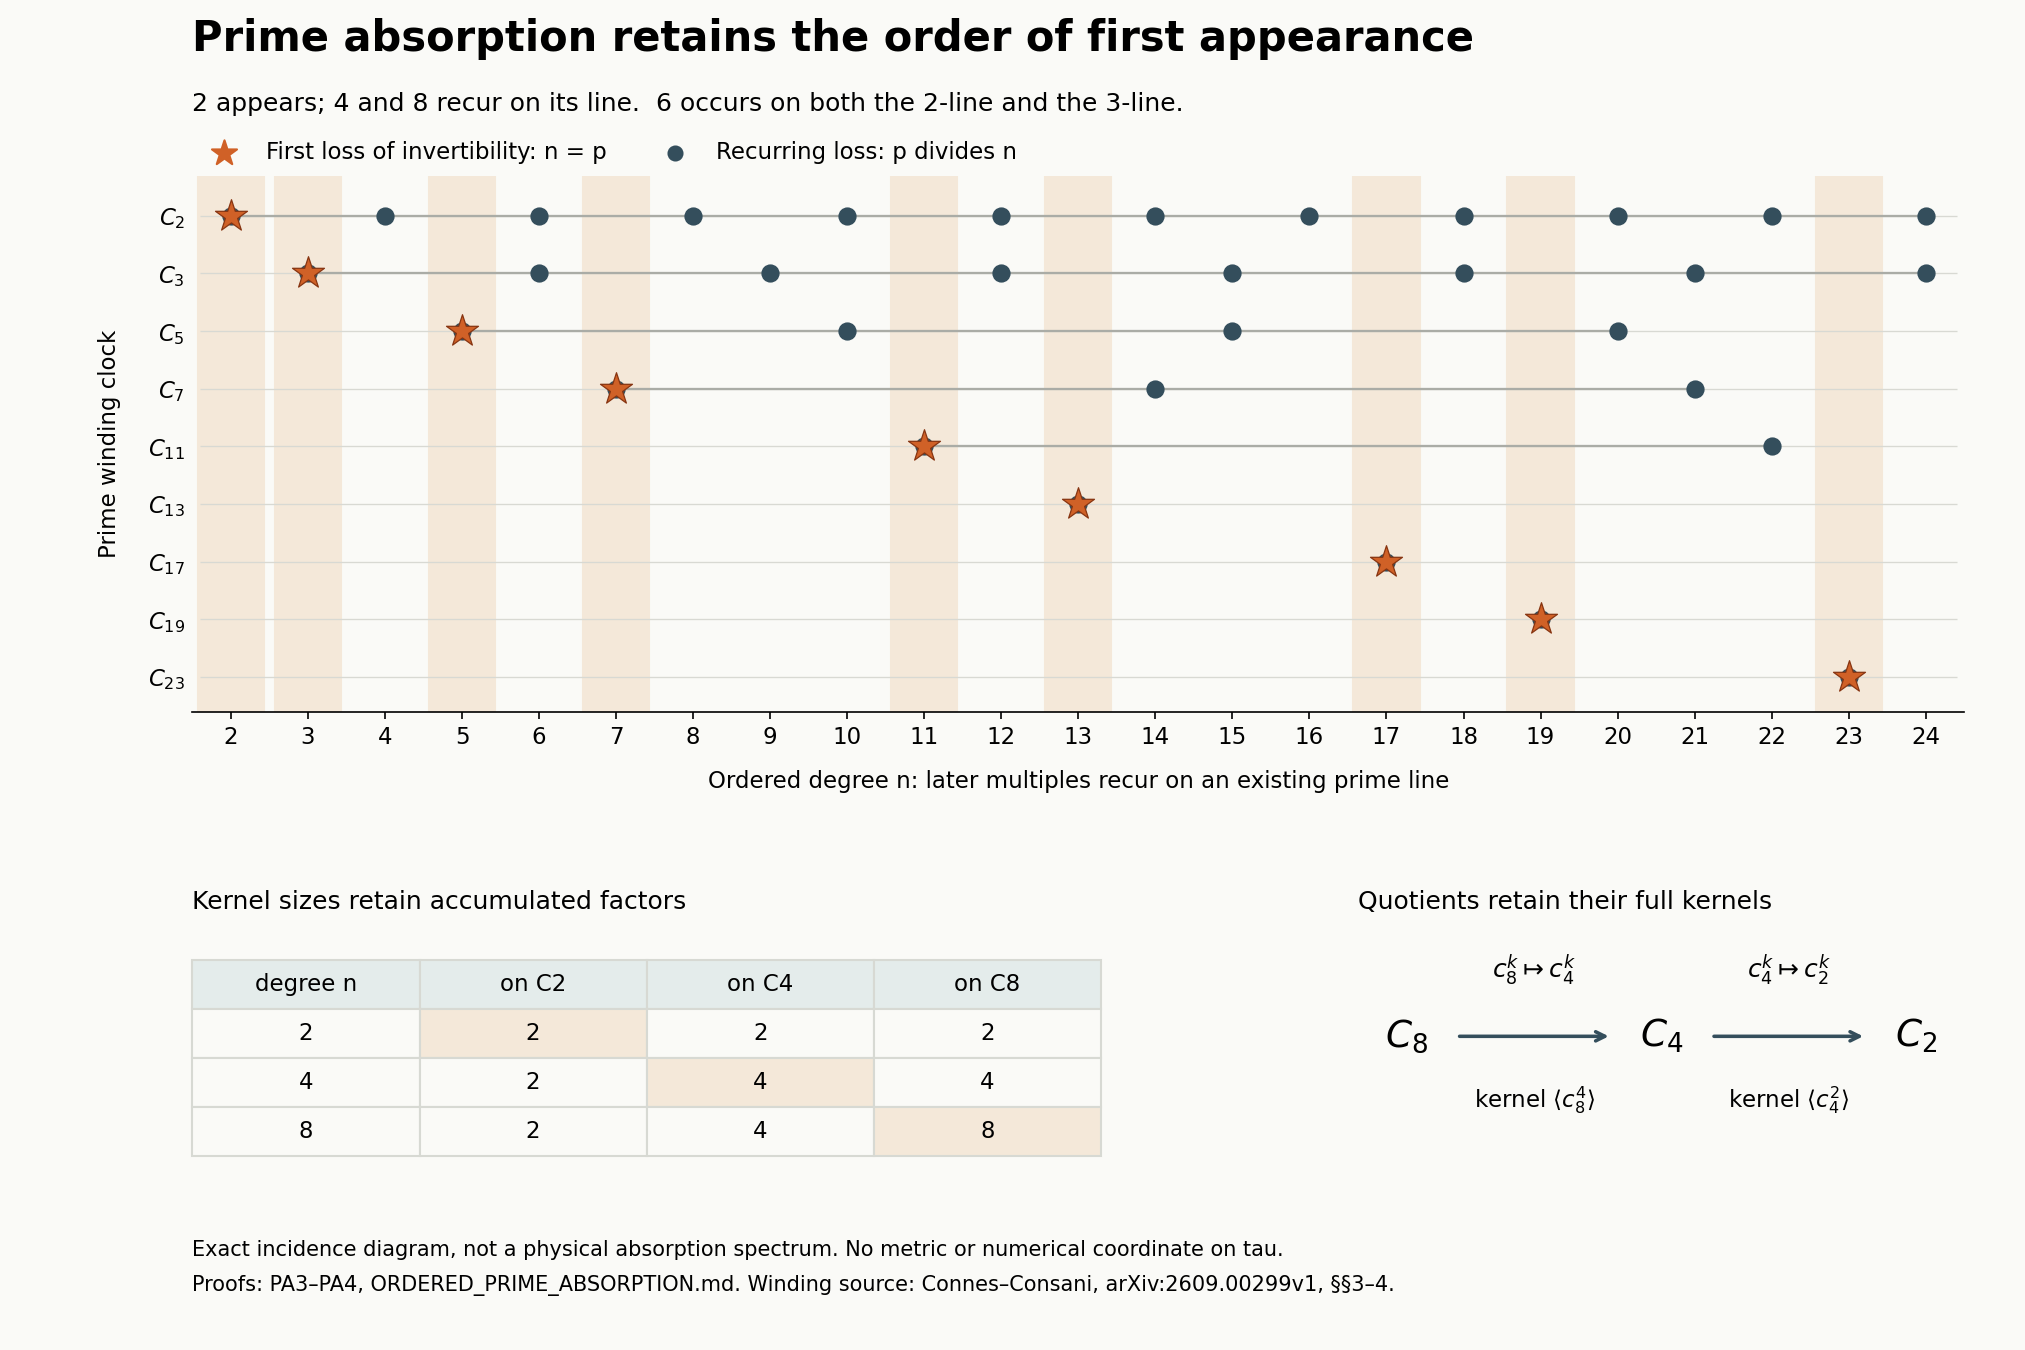
\includegraphics[width=\linewidth]{prime_absorption_clock_20260924/ORDERED_ABSORPTION.png}
\caption{Ordered prime absorption and retained prime-power depth}
\end{figure}

Figure 1. Each row is a prime clock. A star is its first noninvertible positive degree; later dots are recurring losses on the same clock. The lower panel retains the kernel sizes on the 2, 4 and 8 clocks. The horizontal coordinate is the supplied integer winding-step count, not a coordinate on tau. Full proofs: PA3--PA4. Figure source: \nolinkurl{render_ordered_absorption.py}.

\subsection{PA4. The repeated factors are retained by the clock tower}\label{pa20260924-pa4.-the-repeated-factors-are-retained-by-the-clock-tower}

For \(n>0\), let \(v_p(n)\) be the largest integer \(v\ge0\) for which \(p^v\mid n\). It exists because \(p^v\ge2^v\ge v+1\) is eventually greater than \(n\). Write the full factorization \(n=p^{v_p(n)}u\), with \(p\nmid u\). Then \[
\ker([n]:C_{p^a}\to C_{p^a})
=\left\langle c_{p^a}^{\,p^{\max(a-v_p(n),0)}}\right\rangle,
\quad
|\ker[n]|=p^{\min(a,v_p(n))},\qquad a\ge1.
\tag{PA4.1}
\] Indeed \(c_{p^a}^k\) lies in the kernel exactly when \(p^a\mid p^{v_p(n)}uk\). If \(v_p(n)\ge a\), every \(k\) works. Otherwise \(u\) is invertible modulo \(p^{a-v_p(n)}\) by Bezout, giving \(p^{a-v_p(n)}\mid k\). Counting this subgroup proves its stated order. For \(n=0\) the map is constant and the kernel is all \(C_{p^a}\); zero is excluded from positive arrivals. For negative degree the kernel agrees with that of its absolute value, while the original signed degree is still retained.

Consequently, the largest \(a\) for which the whole \(C_{p^a}\) is killed is exactly \(v_p(n)\). At \(n=2,4,8\), the kernel-size triples for \(C_2,C_4,C_8\) are respectively \[
(2,2,2),\qquad(2,4,4),\qquad(2,4,8).
\] They share the first 2-line while their repeated factors are fully distinguished.

Repeatedly choose a prime divisor of \(n>1\) and divide by it. Each division decreases the positive integer, so the process terminates at 1 and supplies a factorization. The multiplicities are independent of the choices. To prove this, if \(p\mid ab\) and \(p\nmid a\), an equation \(xp+ya=1\) multiplied by \(b\) gives \(p\mid b\). Hence a prime dividing a product divides a factor. Compare two prime factorizations, match a prime from one with an equal prime in the other, cancel it, and repeat. Thus \[
n=\prod_{p\mid n}p^{v_p(n)}
\] with every repetition retained. This is classical unique factorization proved here, not a new theorem about primes.

It also reconstructs the whole clock. Put \(n_p=p^{v_p(n)}\) and \(N_p=n/n_p\). Then \[
C_n\longrightarrow\prod_{p\mid n}C_{n_p},\qquad c_n^k\longmapsto(c_{n_p}^k)_{p\mid n}
\tag{PA4.2}
\] has the explicit inverse \[
(c_{n_p}^{a_p})_{p\mid n}\longmapsto
c_n^{\sum_{p\mid n}a_pu_pN_p},\qquad
u_pN_p+v_p' n_p=1.
\] Here \(u_p,v_p'\) are Bezout coefficients, with the prime valuation still denoted \(v_p(n)\). Modulo \(n_p\), the indicated sum is \(a_p\): its other terms contain \(n_p\), while \(u_pN_p\equiv1\pmod {n_p}\). Conversely an exponent zero modulo all \(n_p\) is divisible by their product \(n\), by the prime-divisor result just proved. These facts prove both inverse identities and well-definedness. The isomorphism preserves the marked state and diagonal winding action.

\subsection{PA5. The full source mirror forces an even winding period}\label{pa20260924-pa5.-the-full-source-mirror-forces-an-even-winding-period}

The prime-clock obstruction also gives the precise ordinary prime point in the recovered ring \(R\). Its action map \[
R\longrightarrow\operatorname{End}_{\mathrm{Ab}}(C_p),\qquad [n]\longmapsto[n]_p
\] uses the induced map \([n]_p(c_p^k)=c_p^{nk}\) on the quotient and is surjective: every endomorphism is determined by the image \(c_p^n\) of its generator. Its kernel is \(pR\) by PA3.1. Every nonzero class has an inverse by the same Bezout calculation, so \(R/pR\) is a field and \(pR\) is maximal, hence prime. This is the annihilator of the entire prime clock.

These, together with \((0)\), are all prime ideals of \(R\). Through PA2's ring isomorphism, a nonzero ideal has a least positive integer \(d\); division with remainder shows each of its elements is divisible by \(d\), so it is \(d\mathbb Z\). The value \(d=1\) gives the whole ring and is excluded by properness. If \(d=ab\) with \(1<a,b<d\), then \(ab\) lies in this ideal and neither factor does, so it is not prime. The prime values of \(d\) give the ideals just proved maximal. The zero ideal is prime because a product of two nonzero integers is nonzero. This proves the stated classification. It concerns \(\operatorname{Spec}R\), with its exact source in the winding endomorphisms; it does not replace the full tau-lattice spectrum or identify its additional support points with ring elements.

The winding quotients in PA2 do not discard the original \(H\): it remains in the exact sequence in PA1. To perform finite observations retaining the mirror and \(H\) together, use \[
G_{2p}=G/\langle T^{2p}\rangle\cong C_{2p}\times C_4,
\qquad M_{2p}=G_{2p}\sqcup\{0_M\}.
\] The quotient has \(8p\) units, all four elements of \(H\) remain distinct, and \[
A_{2p}([m]_{2p},[k]_4)=([-m]_{2p},[2m-k]_4).
\] Changing \(m\) by \(2p\) changes \(2m\) by \(4p\), proving well-definedness. Also \(A(T^{2p})=T^{-2p}\), proving that the quotient map intertwines the mirrors.

The extra factor 2 has an exact source reason. Let \(K\le G\) be mirror invariant and retain \(H\) injectively in \(G/K\), namely \(K\cap H=\{1\}\). For \(g=T^mJ^k\in K\), \[
gA(g)=\epsilon^m\in K\cap H.
\] Therefore \(m\) must be even. In particular for odd \(p\), the relation \(T^p=1\) alone is not mirror invariant: its mirror is \(\epsilon T^{-p}\), forcing \(\epsilon=1\) if both were imposed. Its smallest invariant enlargement is \(\langle T^p,\epsilon\rangle\); this gives \(C_p\times C_2\) and loses the original nontrivial sign. We retain it by using period \(2p\).

The map to the prime clock is \[
\rho_p:G_{2p}\to C_p,\quad ([m]_{2p},[k]_4)\mapsto c_p^m.
\] It is surjective; its kernel consists of \(m=0,p\pmod{2p}\) with arbitrary \(k\), hence has eight elements. Its mirror is inversion on \(C_p\).

For odd \(p\), the full coordinates are equivalently \((m\bmod p,m\bmod2,k\bmod4)\); injectivity follows from coprimality, and surjectivity from equal finite cardinality. The mirror is \((r,s,k)\mapsto(-r,s,2s-k)\). At \(p=2\) retain \(C_4\times C_4\): \(C_4\) cannot be replaced by \(C_2\times C_2\), whose elements all have order at most 2. Period 2 already preserves the mirror at this prime; period 4 is the uniform choice, not a claimed minimum there. None of these finite observations alters the source's restriction to odd Frobenius powers.

\subsection{PA6. A faithful finite-prime receiver with a derived common modulus}\label{pa20260924-pa6.-a-faithful-finite-prime-receiver-with-a-derived-common-modulus}

Retain both complex branches and every prime label: \[
D_p=\{(z,j):z^{2p}=1,\ j=i\text{ or }-i\},
\qquad D=\coprod_{p\text{ prime}}\{p\}\times D_p.
\] The source evaluates \(\epsilon\) as \(-1\), and \(J^2=\epsilon\) requires \(j^2=-1\) (Connes--Consani, Proposition \texttt{prop:points\_X\_K}, original lines 619--678). Each pair therefore gives the exact multiplicative map \[
\chi_{p,z,j}:M\to\mathbb C,\qquad
\chi(0_M)=0,\quad
\chi(\epsilon^aT^mJ^b)=(-1)^az^mj^b.
\] All defining relations hold: \(j^2=-1\), \(j^4=1\), and complex multiplication commutes. Since \(z^{2p}=1\), it factors through \(M_{2p}\). No map from tau to the number 1 is used.

Set \(\ell_p=\operatorname{lcm}(2p,4)\), which is \(4p\) for odd \(p\) and 4 for \(p=2\). Every unit value satisfies \[
\chi(g)^{\ell_p}=1.
\] Thus it is algebraic and has absolute value 1. Every complex embedding of its number field preserves the equation \(x^{\ell_p}=1\), so every algebraic conjugate has absolute value 1 as well. This common modulus follows from finite order and was not imposed on the infinite source.

The simultaneous receiver \[
E:M\to\mathbb C^D,\qquad E(g)(p,z,j)=\chi_{p,z,j}(g)
\tag{PA6.1}
\] is injective and multiplicative, with coordinatewise multiplication in its target. To prove injectivity, suppose the images of \(T^mJ^k\) and \(T^nJ^h\) agree. Evaluate at \(z=1,j=i\) to obtain \(k=h\pmod4\). Then \(z^{m-n}=1\) for every \(2p\)-th root and every prime \(p\). If \(m-n\ne0\), choose a prime divisor \(p\) of \(|m-n|+1\), using the least-divisor proof in PA3. This prime does not divide \(m-n\). The value \(z=\exp(\pi i/p)\), of exact order \(2p\), contradicts \(z^{m-n}=1\). Thus \(m=n\). Finally \(E(0_M)\) is identically zero, whereas each unit image is nowhere zero. This proves the assertion on all of \(M\).

The receiver is compatible with the full mirror: \[
E(Ag)(p,z,j)=E(g)(p,-z^{-1},-j).
\tag{PA6.2}
\] Indeed \((-z^{-1})^{2p}=1\), and \(-j\) is the other allowed branch. For \(g=T^mJ^k\), its left side is \(z^{-m}j^{2m-k}\); its right side is \((-z^{-1})^m(-j)^k\). They agree by \(j^2=-1\) and \(j^{-1}=-j\). Both sides vanish on \(0_M\).

For the source's positive odd power map \(F_r(g)=g^r\), \(F_r(0_M)=0_M\), \[
E(F_rg)(p,z,j)=E(g)(p,z^r,j^r).
\] Oddness retains \(j^r\in\{i,-i\}\) and \(F_r(\epsilon)=\epsilon\). This equality follows by raising the complete value to its \(r\)-th power; the factor \((-1)^a\) remains. It is a point-level monomial comparison, not a new theorem identifying an arithmetic cohomology.

For winding translation \(\mu_r(g)=T^rg\), with \(0_M\) fixed, the exact formulas are \[
E(\mu_rg)(p,z,j)=z^rE(g)(p,z,j),
\quad A\mu_r=\nu^r\mu_{-r}A,
\quad \nu(g)=\epsilon g,
\] with \(\nu(0_M)=0_M\). These follow from \(A(T^r)=\epsilon^rT^{-r}\). In particular the mirror-translated receiver is \((-1)^rz^{-r}E(Ag)\). Translations are bijections, \(\mu_r\mu_s=\mu_{r+s}\), but for \(r\ne0\) they are not unital monoid maps because \(\mu_r(1)=T^r\ne1\).

\subsection{PA7. Complete additive scope of the receiver}\label{pa20260924-pa7.-complete-additive-scope-of-the-receiver}

Faithfulness in PA6 is a theorem on the original monomials and absorbing element. Its complex-linear extension on the separately constructed group algebra has the exact kernel \[
\ker\bigl(\mathbb C[G]\to\mathbb C^D\bigr)=(1+J^2).
\tag{PA7.1}
\] Here addition belongs to the group algebra, not tau. To prove the assertion, write an arbitrary finite sum as \[
f=\sum_mT^m(a_{m,0}+a_{m,1}J+a_{m,2}J^2+a_{m,3}J^3).
\] Vanishing at \(j=i\) and at \(j=-i\) gives two Laurent polynomials in \(z\) that vanish at all finite-prime parameters. There are infinitely many distinct such parameters: a finite list of primes cannot contain every prime divisor of their product plus 1, by PA3, and \(\exp(\pi i/p)\) are distinct for distinct primes. A nonzero polynomial of degree \(d\) has at most \(d\) distinct roots, proved by repeated division by its linear factors. Multiplying a Laurent polynomial by a sufficiently large power of \(z\) therefore shows both Laurent polynomials are zero. Their coefficients give \[
a_{m,0}-a_{m,2}+i(a_{m,1}-a_{m,3})=0,
\quad
a_{m,0}-a_{m,2}-i(a_{m,1}-a_{m,3})=0.
\] Adding and subtracting gives \(a_{m,0}=a_{m,2}\), \(a_{m,1}=a_{m,3}\). Hence \[
f=(1+J^2)\sum_mT^m(a_{m,0}+a_{m,1}J).
\] Conversely \(1+J^2\) evaluates to zero everywhere, proving both inclusions. Thus the exact faithful additive receiver is the quotient by this ideal, with its projection retained. This does not replace the spherical algebra in PA1.

The finite-prime parameters are dense, but not all, in \(S^1\times\{i,-i\}\). For \(e^{i\theta}\), choose an integer \(k_p\) nearest \(p\theta/\pi\); then \[
|e^{i\theta}-e^{\pi i k_p/p}|\le |\theta-\pi k_p/p|\le\frac{\pi}{2p}.
\] The first inequality follows by integrating \(i e^{it}\) between the two angles. Primes are unbounded by the preceding product-plus-one argument, giving density. The value \(e^{2\pi i\sqrt2}\) is not a root of unity: a finite order would make a positive integer multiple of \(\sqrt2\) an integer. Irrationality of \(\sqrt2\) follows since a coprime equation \(a^2=2b^2\) makes first \(a\), then \(b\), even. This proves properness. These circles describe complex character values; no circle or metric is assigned to tau.

\subsection{PA8. The original zeta function recovered from the ordered births}\label{pa20260924-pa8.-the-original-zeta-function-recovered-from-the-ordered-births}

The birth set in PA3 gives the original Euler factors with all repetitions retained. For a complex variable \(s\) with \(\sigma=\Re s>1\), use the original series \[
\zeta(s)=\sum_{n=1}^{\infty}\exp(-s\log n).
\] Its absolute convergence follows from \(\sum_{n>B}n^{-\sigma}\le\int_B^\infty x^{-\sigma}\,dx
=B^{1-\sigma}/(\sigma-1)\), for integer \(B\ge1\). For the finite birth set \(V_B\), define \[
P_B(s)=\prod_{p\in V_B}\left(1-\exp(-s\log p)\right)^{-1}.
\] Expanding each geometric series is valid because \(p^{-\sigma}<1\). A finite product of absolutely convergent series is absolutely convergent. PA4's unique factorization shows its terms are exactly the original \(n^{-s}\) for integers all of whose prime factors belong to \(V_B\), once each, including the term \(n=1\). Consequently the exact remainder and its bound are \[
\zeta(s)-P_B(s)
=\sum_{\substack{n\ge1:\ \exists\ p>B\ \mathrm{prime},\ p\mid n}}\exp(-s\log n),
\qquad
|\zeta(s)-P_B(s)|\le\frac{B^{1-\sigma}}{\sigma-1}.
\tag{PA8.1}
\] Every omitted integer is greater than \(B\), giving the inequality. Therefore the ordered births and their repeated factors recover the original zeta series on this domain, with an explicit remainder. Nothing has been divided by a Gamma factor, a power of pi, an endpoint factor or a completion multiplier. This computation does not extend the convergence domain or bound zeros in the critical strip.

\subsection{PA9. Exact comparison with the requested purity mechanism}\label{pa20260924-pa9.-exact-comparison-with-the-requested-purity-mechanism}

PA6 proves that every nonzero finite-character value is algebraic and that all its conjugates have absolute value 1. In Deligne's terminology for an algebraic number relative to \(q>1\), this is weight zero because \(q^{0/2}=1\). It is a conclusion about these values, not a choice of radius on the source.

The arithmetic statement to which it must be compared keeps its original factors. Deligne's weight definition at a closed point \(x\) requires Frobenius eigenvalues with \[
|\iota(\alpha_x)|=N(x)^{w/2}
\] for every complex conjugate. His proper smooth conclusion for degree \(i\) has \(|\iota(\alpha)|=q^{i/2}\), where the eigenvalues are roots of \(\det(t\,1-F^*,H^i)\). These are Deligne's results, not conclusions proved by this note. \href{https://www.numdam.org/item/PMIHES_1980__52__137_0/}{Pierre Deligne, \emph{La conjecture de Weil. II}, Definitions 1.2.1--1.2.2 and Corollary 3.3.9}.

The exact gain over a freely selected common-modulus character set is PA5--PA6: finite prime clocks give a faithful monomial receiver with that modulus, and the source mirror, sign and branch are retained. No Frobenius action on an RH-detecting arithmetic \(H^1\) has been identified with these evaluations here. The weight-one factor \(N(x)^{1/2}\) has therefore not been obtained or suppressed. The original zeta calculation currently has the proved domain in PA8.

\subsection{PA10. What the single construction retains}\label{pa20260924-pa10.-what-the-single-construction-retains}

The full object used throughout is the signed winding group at the fixed support, its winding quotient, all finite quotient clocks and compatible degree maps, together with the ordered filtration \((V_n,H_n)\), the signed quotients \(M_{2p}\) and their joint receiver \(E\). Each new component is linked by the explicit maps proved above. A hidden composite still has its full clock and its arrival position. Its repeated prime factors remain in PA4's compatible kernels and reconstruction maps.

Thus ``2 is first; 4 is already covered'' is an exact statement of this construction. Replacing its ordered filtration by only the set of prime divisors would change the observation. The first-appearance rule, multiplicity tower, faithful signed receiver and original Euler series are the proved consequences retained together here.

\subsection{Provenance and reproducibility}\label{pa20260924-provenance-and-reproducibility}

\begin{itemize}

\item
  \textbf{User:} sequential prime visibility, absorption interpretation, retention of tau's \(Z_1\) type and the no-parity source distinction. Exact input is retained privately beside this file, without converting speculative statements from the pasted conversation into premises.
\item
  \textbf{Alain Connes and Caterina Consani:} original geometric space, generic algebra, imaginary generator, twisted chart restrictions and mirror; arXiv:2609.00299v1. Read the original author TeX at the precise ranges in \nolinkurl{SOURCE_READING_USE_PRIVATE.json}.
\item
  \textbf{Pierre Deligne:} the quoted weight target and cohomological purity theorem, \emph{La conjecture de Weil. II}, IHÉS 52 (1980), 137--252. The local French TeX is a transcription, not author-supplied TeX. The historically retained English transcription is \href{https://github.com/KokunoYumeto/zeta-function-research-reader/blob/492a44c2938cc6f5e3c41105567492a8fa528c8c/workbenches/splitzero-tandem/continuations/20260919-observation-responses-first-allocation/prior_intakes/supporting_sources/D032_FULL_EN.tex}{available at the pinned programme edition}; its known reciprocal-characteristic-polynomial error is not used. The French transcription controls PA9.
\item
  \textbf{This task:} PA1--PA10's connecting calculations and complete elementary proofs; independently checked clock and signed-character derivations. The underlying cyclic quotient theory, unique factorization and Euler product are classical.
\item
  \nolinkurl{render_ordered_absorption.py} reproduces the illustration. \nolinkurl{check_clock_maps.py} checks finite instances of the displayed maps and outputs; its checks supplement the proofs and are not substituted for them.
\end{itemize}

The earlier source-definition note remains in \texttt{../foundations/user\_definitions\_20260924/}. This construction does not reinstate its withdrawn addition on tau or assert an isomorphism with the entire support-lattice programme. The cumulative TeX includes this complete note; older PDFs are not represented as rebuilt editions.
